\section{Case Studies}
\label{case-studies}

% All are built with our Vue plugin and
% pure client-side applications with no servers
% involved other than those interfaced with below the Graffiti API.

% The first demonstrate interoperability.
% The latter demonstrate how ``weird'' social applications
% can become when there is not central moderator.
The case studies below demonstrate the diversity of applications
that can be built on top of the Graffiti API and explore interoperation
between those applications.
The studies also demonstrate some of the unusual design patterns that
Graffiti makes possible when the boundaries between applications
are fuzzy and no one is really in control.

Other than the interoperation we describe, no \emph{unexpected}
interoperation occurs, thanks to our channels concept.
For example, group chat messages do not show up as posts on
a microblogging site even though both use similar object schemas,
because they are each posted to different channels.

All of the applications are written with pure client-side code on
top of the Graffiti Vue plugin.

\subsection{Glitter and The Glue Factory}
%DK Why lump these together?   Describe Glitter first (and discuss how easy it is to implement) than describe Gloof and explain how they interoperate

The following example demonstrates how a community-specific application,
%DK I would call this a social site rather than an application (and explain why).
\emph{The Glue Factory}\footnote{
\url{https://gluefactory.live}, Source: \url{https://github.com/horseyhouse/glue-factory}
}, can interoperate with a general-purpose application, \emph{Glitter}\footnote{
\url{https://glitter.graffiti.garden}, Source: \url{https://github.com/graffiti-garden/glitter}
},
without the explicit permission of Glitter.
Not all of the community-specific features on The Glue Factory
translate to Glitter, and not all of the interconnectedness on Glitter
is forced upon The Glue Factory.
Still, there is enough interoperation between the two to be meaningful.

\emph{Glitter} is a text-centric microblogging platform
where users can post, follow, reply, and change their display name.
Replies are threaded and, like Twitter, appear in the replier's followers' feeds in addition to the reply thread.
There is also a directory that users can add themselves to,
so others can find them.
%DK Is the directory glitter specific?   why?   finding users seems important for most applicatoins.

\emph{The Glue Factory} is an application made for a local
venue to share event flyers.
The flyers are displayed in a grid, similar to Instagram,
but there is just one feed, collectively curated by
the application's fixed set of venue organizers.
Flyers can be replied to, but the organizers may remove replies they disapprove of.

Importantly, The Glue Factory lets
top-level repliers ``crosspost'' their replies
to Glitter, effectively sharing the flyer like a Quote Tweet.
Glitter does not support images and so only the
event description appears.
Replies to the crosspost made on Glitter also appear on The Glue Factory
and vice versa, \emph{unless} The Glue Factory's organizers ``remove'' the reply,
in which case it only appears on Glitter, regardless of where it originated.
Additionally, replies to the crosspost made on Glitter appear in the replier's followers'
feeds while replies made on The Glue Factory only appear in the reply thread,
similar to the difference between Instagram-like and X-like replies described in Section~\ref{concepts:channel-replies}.
Some of this interoperation is shown in Figure~\ref{case-studies:fig:gloof-and-glitter}\footnote{
Flyers are blurred for anonymization during review.
}.

\begin{figure*}[h]
    \Description[Two screen shots beside each other.]{Two screen shots that show textual content from the Gloof application being presented in the general purpose Glitter application.}
    \centering
    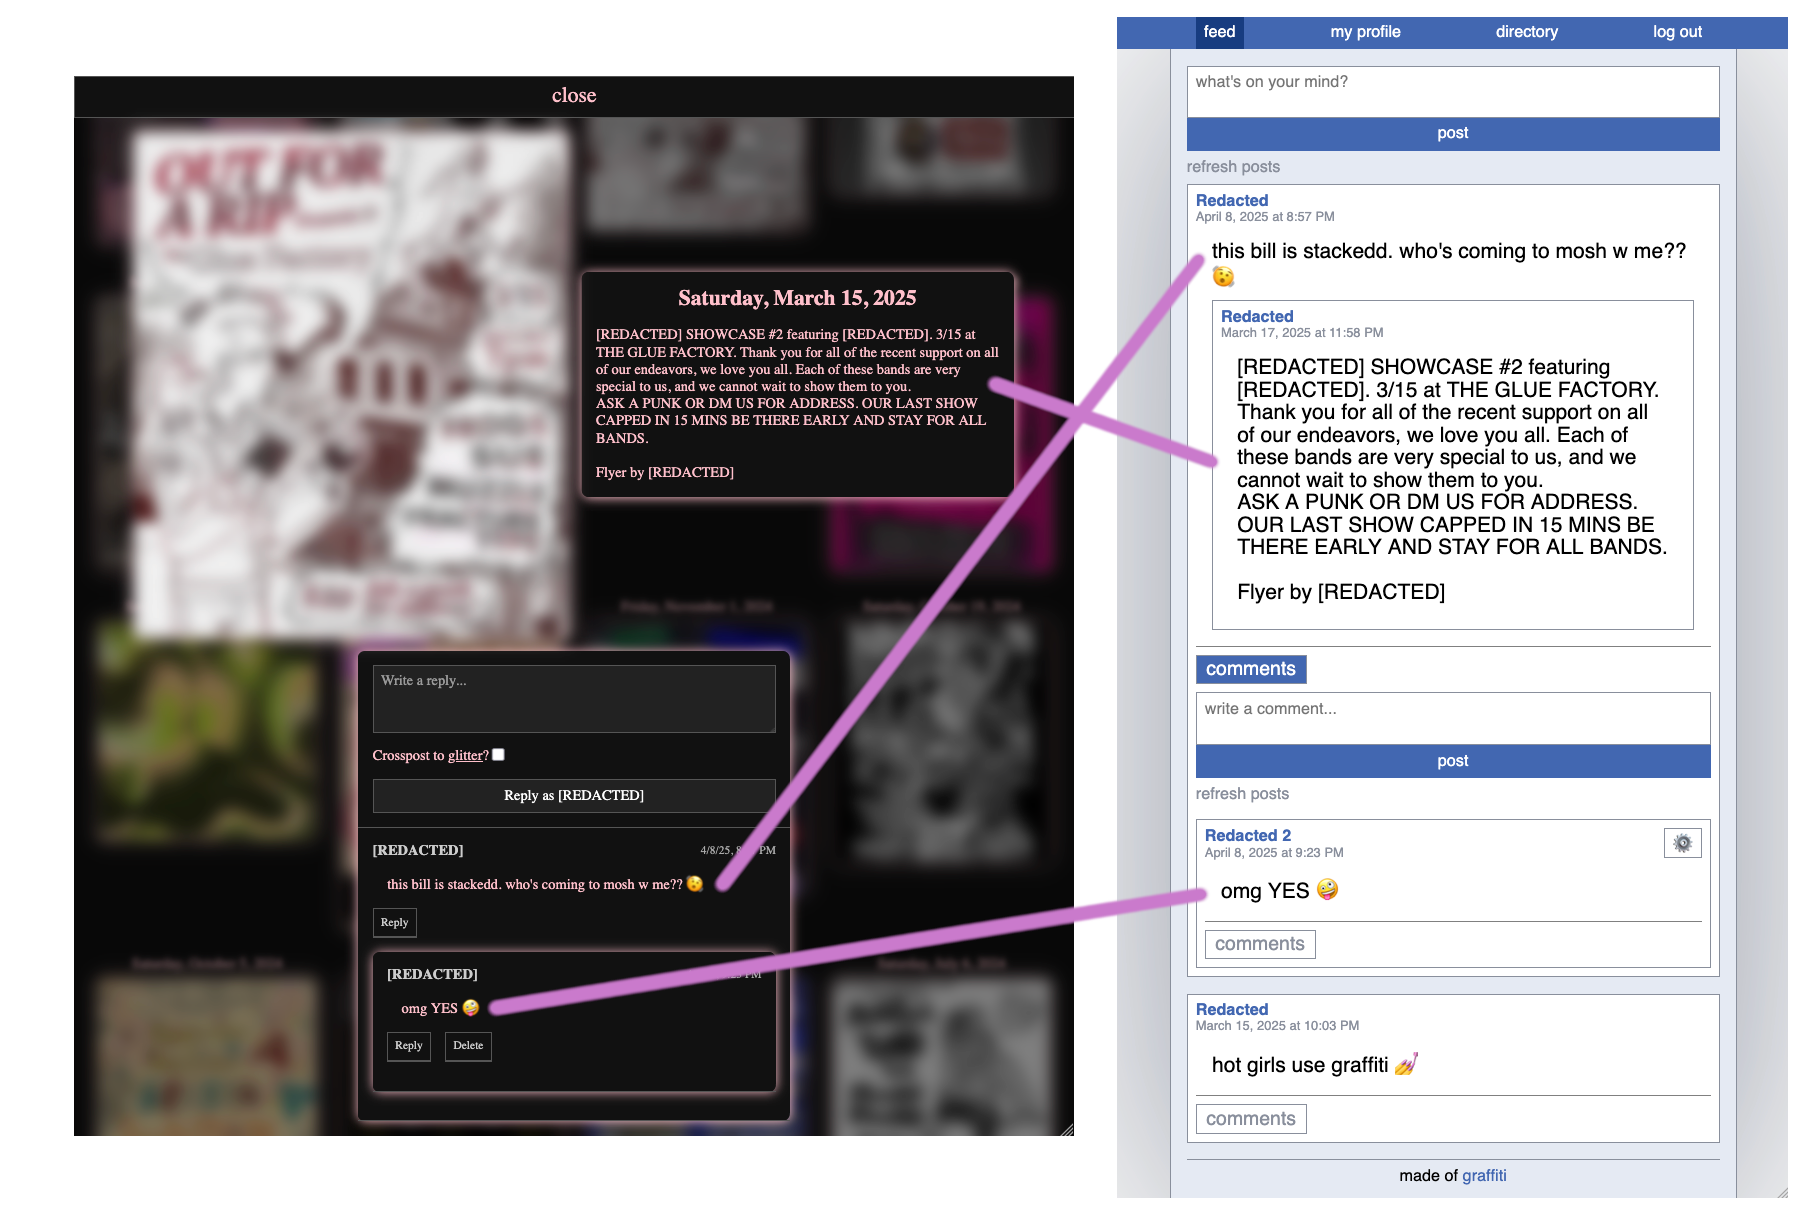
\includegraphics[width=\textwidth]{paper/figures/gloof-and-glitter.png}
    \caption{A reply to a Glue Factory event appears like a quote Tweet on Glitter, with
    interoperating replies.}

    \label{case-studies:fig:gloof-and-glitter}
\end{figure*}
% on Namebook but replies
% to the crosspost show up on both applications,
% allowing repliers ask clarifying questions.
% Namebook does not consider The Gloof's organizers
% moderators of its own site and so replies ``deleted''
% on The Gloof still show up on Namebook.
% Finally, replies made on The Gloof only appear
% in the reply thread while replies made on Namebook
% appear on the user's profile, even if they are in
% reply to posts on The Gloof.

The applications are built out of the objects and channels
shown in Figure~\ref{case-studies:fig:schemas-and-channels}.
Importantly, both applications use the same reply object schema,
and the post object schema used by Glitter is a subset of the flyer
object schema used by The Glue Factory.
This overlap makes interoperation \emph{possible},
but selecting ``crosspost'' in The Glue Factory intentionally collapses the
channel usage of the two applications,
causing the interoperation to actually \emph{happen}.

\begin{figure*}[h]
    \Description[Diagram showing four channels with examples of objects in each.]{Diagram showing that Glitter and Glue Factory each have a channel, each actor and each post has a channel, and an object can be in both the actor and post channels.  }
    \centering
    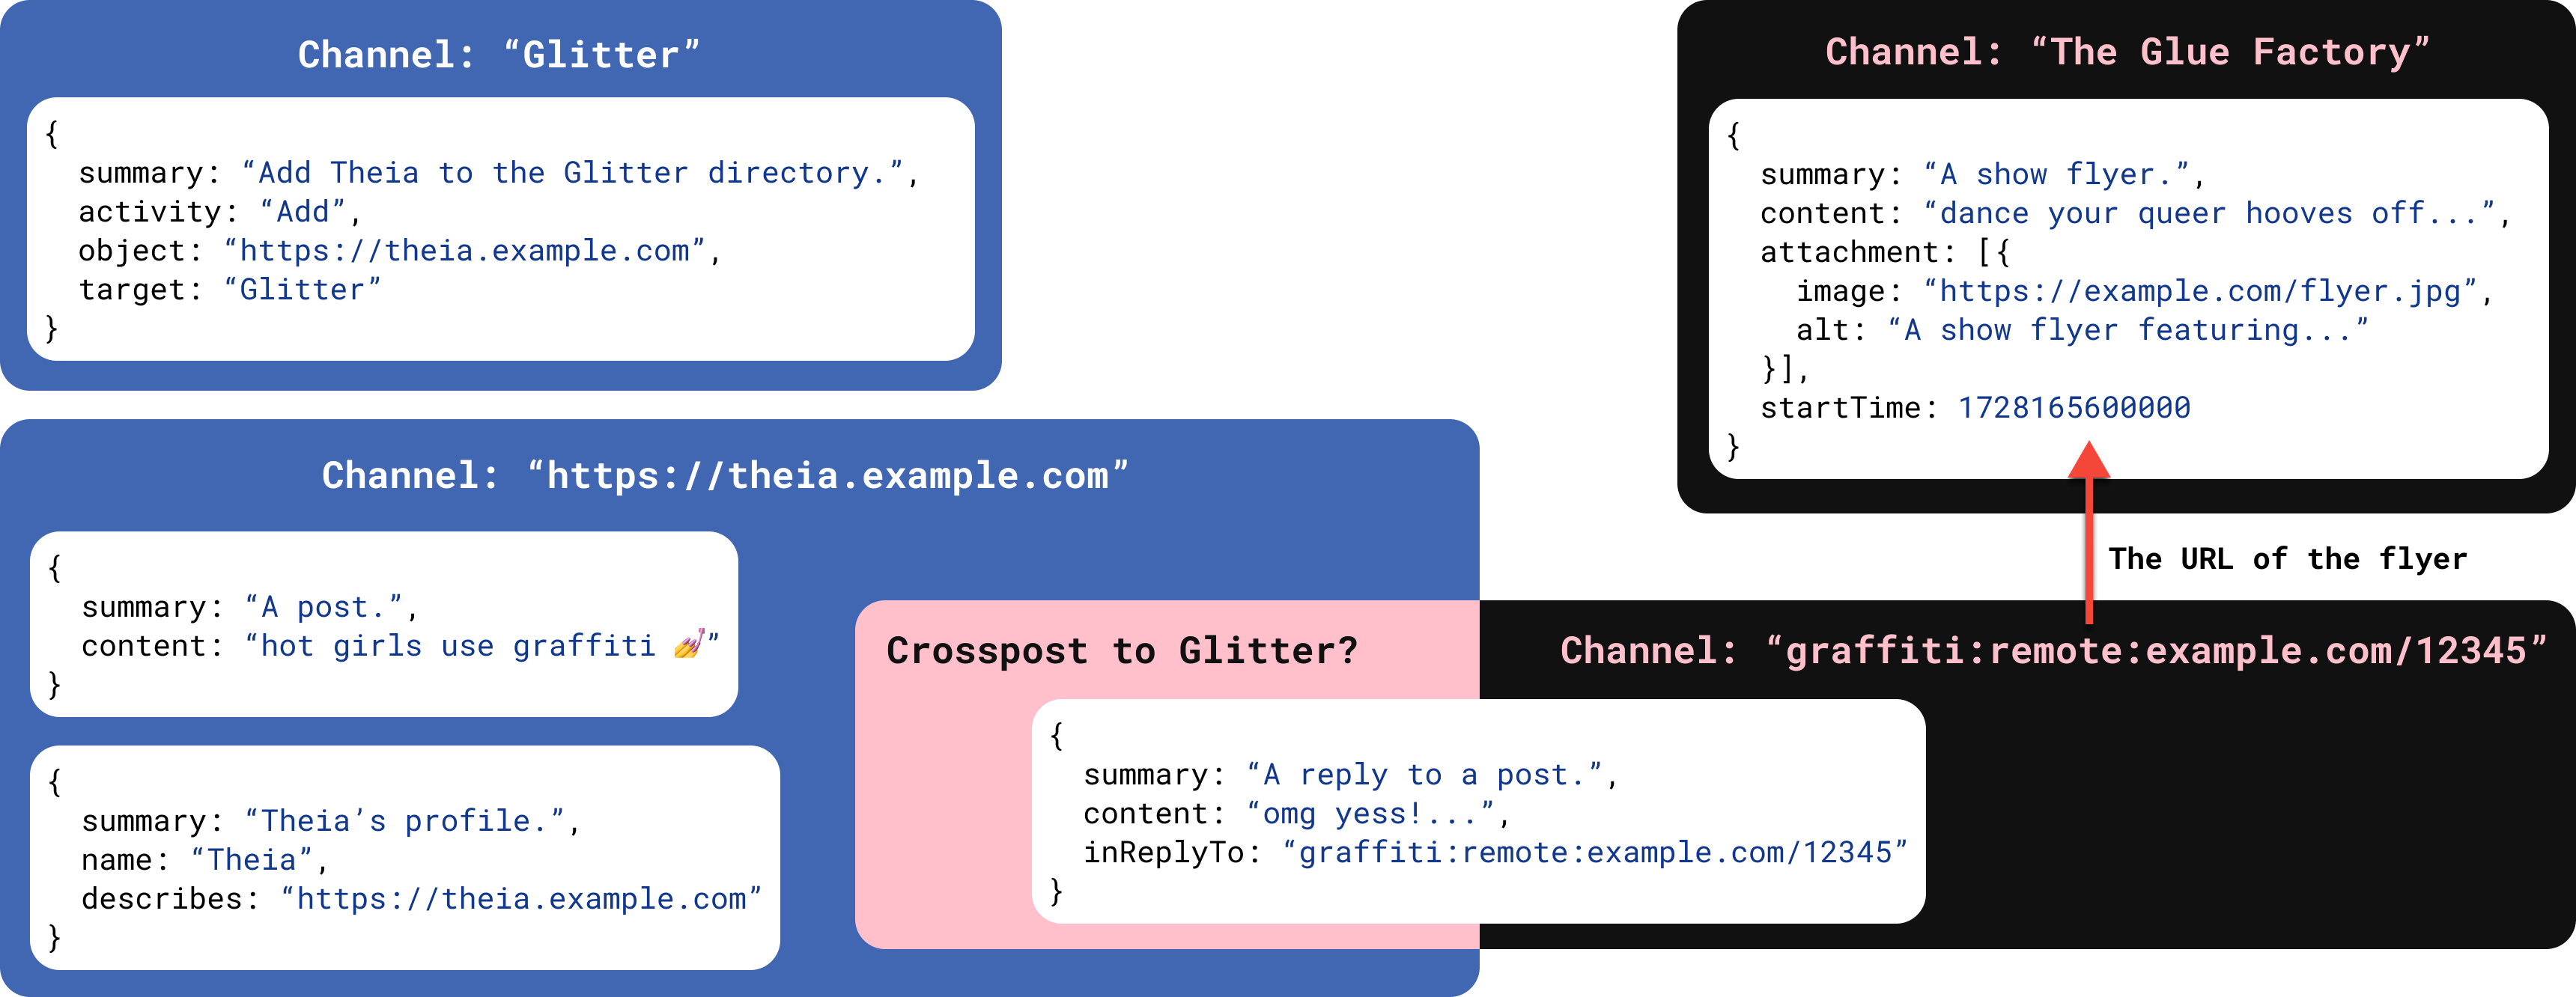
\includegraphics[width=\textwidth]{figures/schemas-and-channels.png}
    \caption{The objects and channels used by Glitter and the Glue Factory, and their overlap}

    \label{case-studies:fig:schemas-and-channels}
\end{figure*}

% Namebook employs four object schemas: posts and replies are represented
% by one schema with \texttt{content}, a \texttt{published} timestamp, and an optional
% \texttt{inReplyTo} link;
% name changes represented by objects with a \texttt{name} and
% \texttt{desribes} property pointing to the actor's URI;
% \texttt{"Follow"} and \texttt{"Add"} activities
% are used for following and adding one's self to the name book respectively
% and each \texttt{target} the relevant actor URI.
% All posts, replies, and name changes are published to the actor's URI
% channel. Replies are also posted to original post's URL channel.
% Finally, \texttt{"Add"} activities are simply posted to the channel \texttt{"namebook"}.

% Gloof employs three object schemas. Replies are identitical to Namebook's,
% while flyers have additional properties \texttt{startTime},
% and \texttt{attachment} for including the flyer image.
% Moderation is done with \texttt{"Remove"} activities that
% target the relevant actor URI.
% Flyer's are posted in the channel \texttt{"gloof"} while
% replies are posted in


% To make this work,
% Namebook posts are posted to the actor's own URI channel,
% as described in Section~ref{}
% Namebook posts under a user's channel as described in section~\ref{concepts:channels}.
% Gloof posts are posted to the channel \texttt{"gloof"} and filtered
% for only their approved.
% Gloof posts can be optionally cross-posted to Namebook.
% Namebook cannot parse the images but can still read the
% text description.
% Additionally, comments on Namebook are Twitter-like
% and available in a replies tab, unlike Gloof comments
% which only show up under the post

One additional note is that flyers posted to The Glue Factory include a \texttt{startTime}
to display event dates.
This metadata is also used to populate a separate calendar application
used by the co-operative that owns the venue space.

% Posts to Gloof can be cross-posted to Namebook.

% Users of [Redacted] can are "cross-posted" to Namebook.
% Comments under than post show up on
% both Namebook and [Redacted]. However,
% Comments on Namebook \emph{also} show up
% in the users profile. THis is not the case
% for comments on Redacted which, like INstagra

% Additionally, on [Redacted] you can delete comments.
% This is not possible on Namebook.

\subsection{Parallax and Provenance}
\label{case-studies:parallax}

%DK perhaps before getting into the crazy bits, talk about how easy it is to implement a basic group chat application ("Grack").   Each group is defined by a channel, and you invite someone to the group by notifyig them about the channel.  There is no admin---anyone in the group can invite others---and no way to remove people without their consent (but you can always create a new group excluding them).  Maybe also describe how you would design a facebook clone ("Gracebook") differently: a user can post content for friends by putting it in their own actorID channel but with an allowlist consisting of their friends.  alternatively they can create a different channel for sharing posts to their friends and invite all friends to subscribe to it.

\emph{Parallax}\footnote{
\url{https://parallax.graffiti.garden}, Source: \url{https://github.com/graffiti-garden/parallax}
} is a real-time group chat application that demonstrates
how, under total reification, it is possible for \emph{every} user to employ a different
moderation scheme.
Specifically,
every user, from their own perspective,
is the sole administrator of \emph{all} group chats (that they know about) with
unilateral control over each group's name and membership.
The messages a user sends in a group can only be seen by the users they explicitly
put on that group's membership list.
However, users can also see the changes that other users
make to their own ``views'' of a group and are given the option
to \emph{voluntarily} incorporate those changes,
as shown in Figure~\ref{case-studies:fig:parallax}.

\begin{figure*}[h]
    \Description[Three screen shots.]{The screen shots on the right show the membership lists for Bob and Alice, which determine what each of them see in their version of the shared chat on the left.}
    \centering
    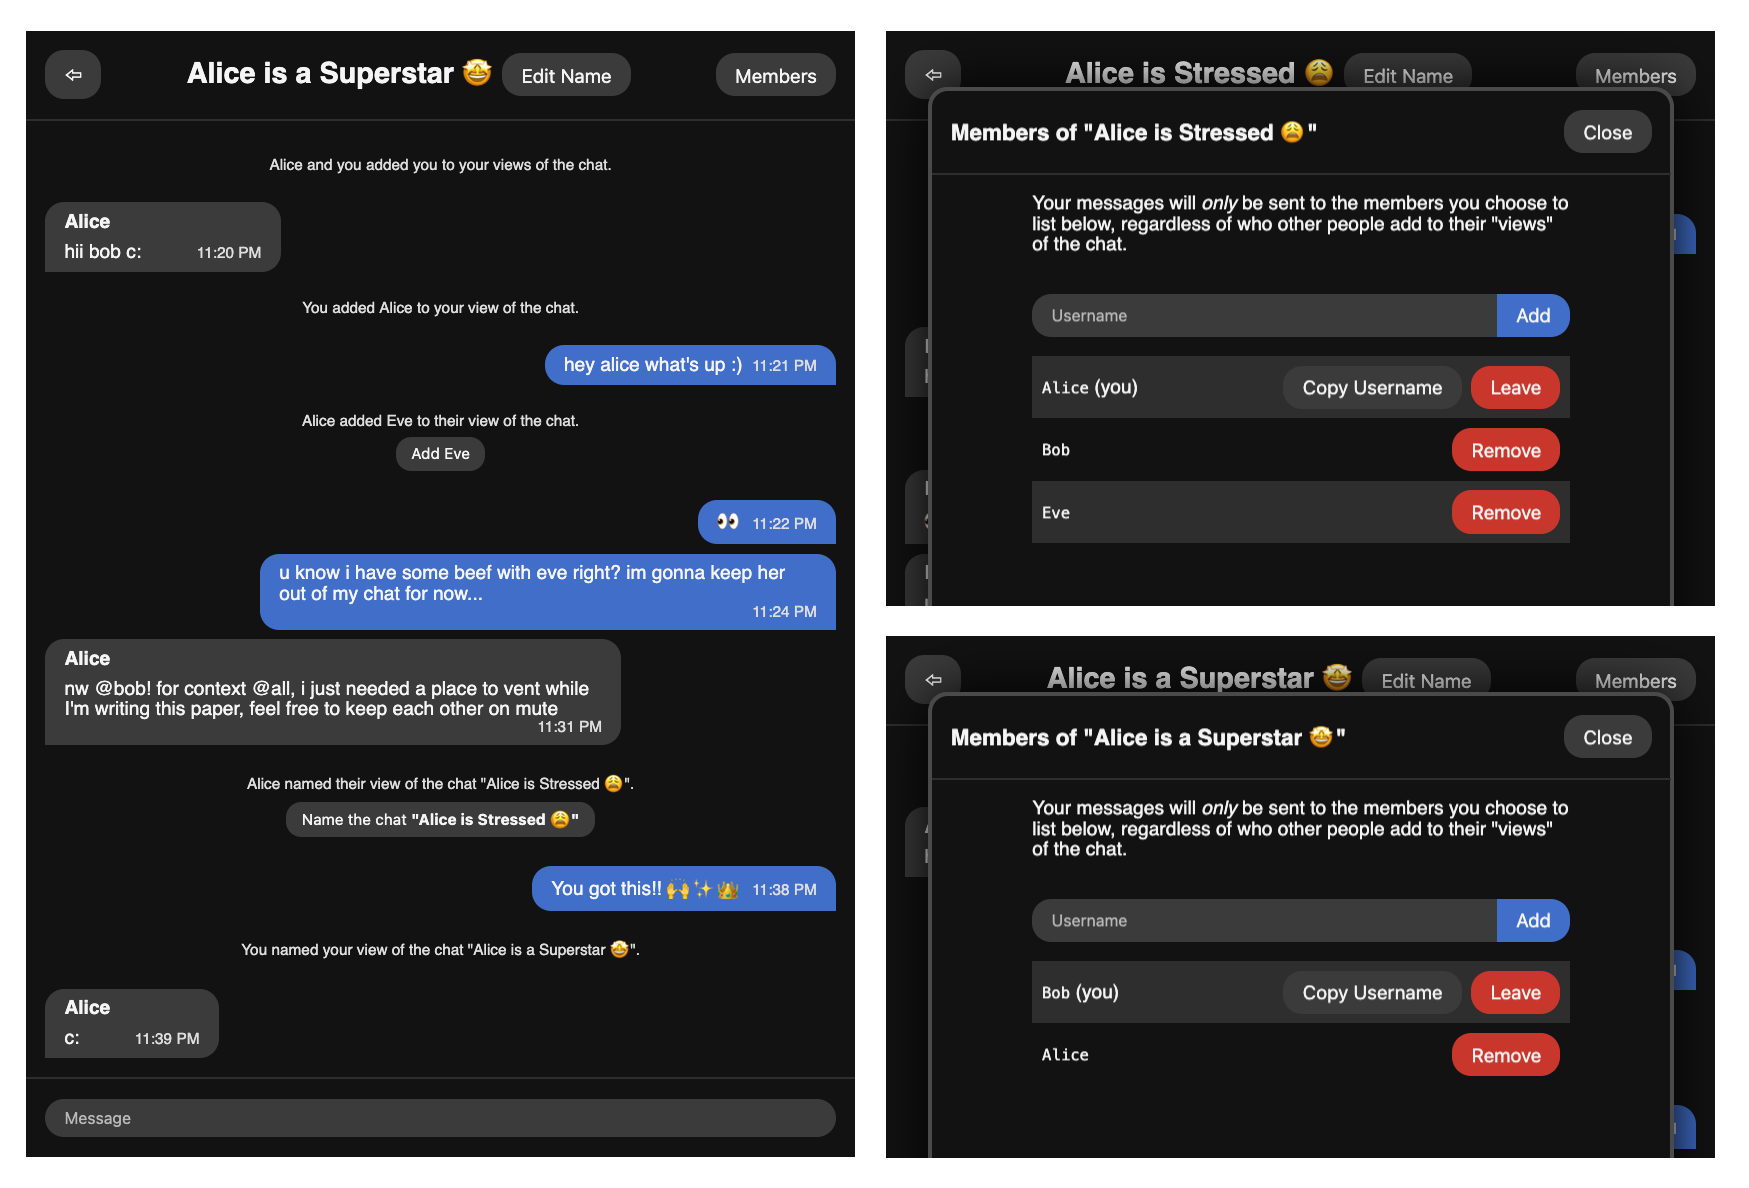
\includegraphics[width=\textwidth]{paper/figures/parallax.png}
    \caption{An interaction on Parallax. On the left is Bob's view of an exchange. On the right are Alice and Bob's \emph{different} membership lists.}

    \label{case-studies:fig:parallax}
\end{figure*}

Under the hood, a group is represented by a random identifier,
generated when the group is created, and also used as the group's channel.
Changes to a group's name are similar to profile name changes on Glitter, only they
\texttt{describe} the group identifier.
A group's membership can be changed with reified \texttt{"Add"}
and \texttt{"Remove"} activities.
Messages use the same object schema as posts on Glitter,
only they have \texttt{allowed} lists, which are determined
by aggregating the user's own \texttt{"Add"} and \texttt{"Remove"} activities
to determine the group membership state.

Of course, complete independence is not always desirable:
work usually done by just one group administrator must, in Parallax,
be done by every single group user.
We use Parallax to demonstrate an extreme,
but it can be
% transformed
% but by changing X lines of functional code,
transformed into a more reasonable (but more restrictive) application called \emph{Provenance}\footnote{
\url{https://provenance.graffiti.garden}, source code is in the parallax repository.
},
where a group's administrator is the  \emph{creator} of the group chat.
%DK not sure what this means.   how does being the creator give them administrator privileges?   and was does admin privilieges mean given adversarial interoperability?

% Provenance determines the \texttt{allowed} list on a user's messages
% by aggregating the \texttt{"Add"} and \texttt{"Remove"} activities made by the first
% actor to post in the chat.

Parallax and Provenance both interoperate,
but some messages sent from one will not be seen in the other
according to their unequal membership lists. However, this messiness is already present and tolerable
in messaging applications like Signal, where users can block other group members,
and email, where any reply can be sent to a different set of recipients.
There is exciting work to be done learning what interfaces make
Graffiti's inevitable assymetry most accessible and engaging.

% While the previous case study demonstrates
% how a user might choose different settings
% \emph{between} applications.
% Here there are settings \emph{within} the application.

% This and the following app are extreme.
% In many cases the user would not to
% have fine grained control over group
% membership and would like to delegate
% some of that work to, say, the person
% who created the groupchat.
% Additional layers like this are possible
% but it is always possible for an application
% like this one to interoperate with
% more traditional ones.

% Maybe show traditional chat app and how
% it interoperates?

\subsection{Wikiffiti}

Wikiffiti\footnote{
\url{https://wikiffiti.graffiti.garden}, Source: \url{https://github.com/graffiti-garden/wikiffiti}
} is a Wikipedia-like application that demonstrates that
collaborative editing in Graffiti is possible,
even though an actor can only mutate their own objects.
Additionally, unlike Wikipedia,
every user on Wikiffiti can choose which other users have ``permission'' to edit an article,
\emph{retroactively} undoing edits by unpermissioned users,
as shown in Figure~\ref{case-studies:fig:wikiffiti}.
The user can only control which users' edits \emph{they} see, not exert any global control---so different users may end up seeing different pages.

\begin{figure*}[htb]
    \Description[Four screen shots showing changes to a Wikifitti page.]{Four screen shots showing how the actions of successive edits evolve the text as viewed.}
    \centering
    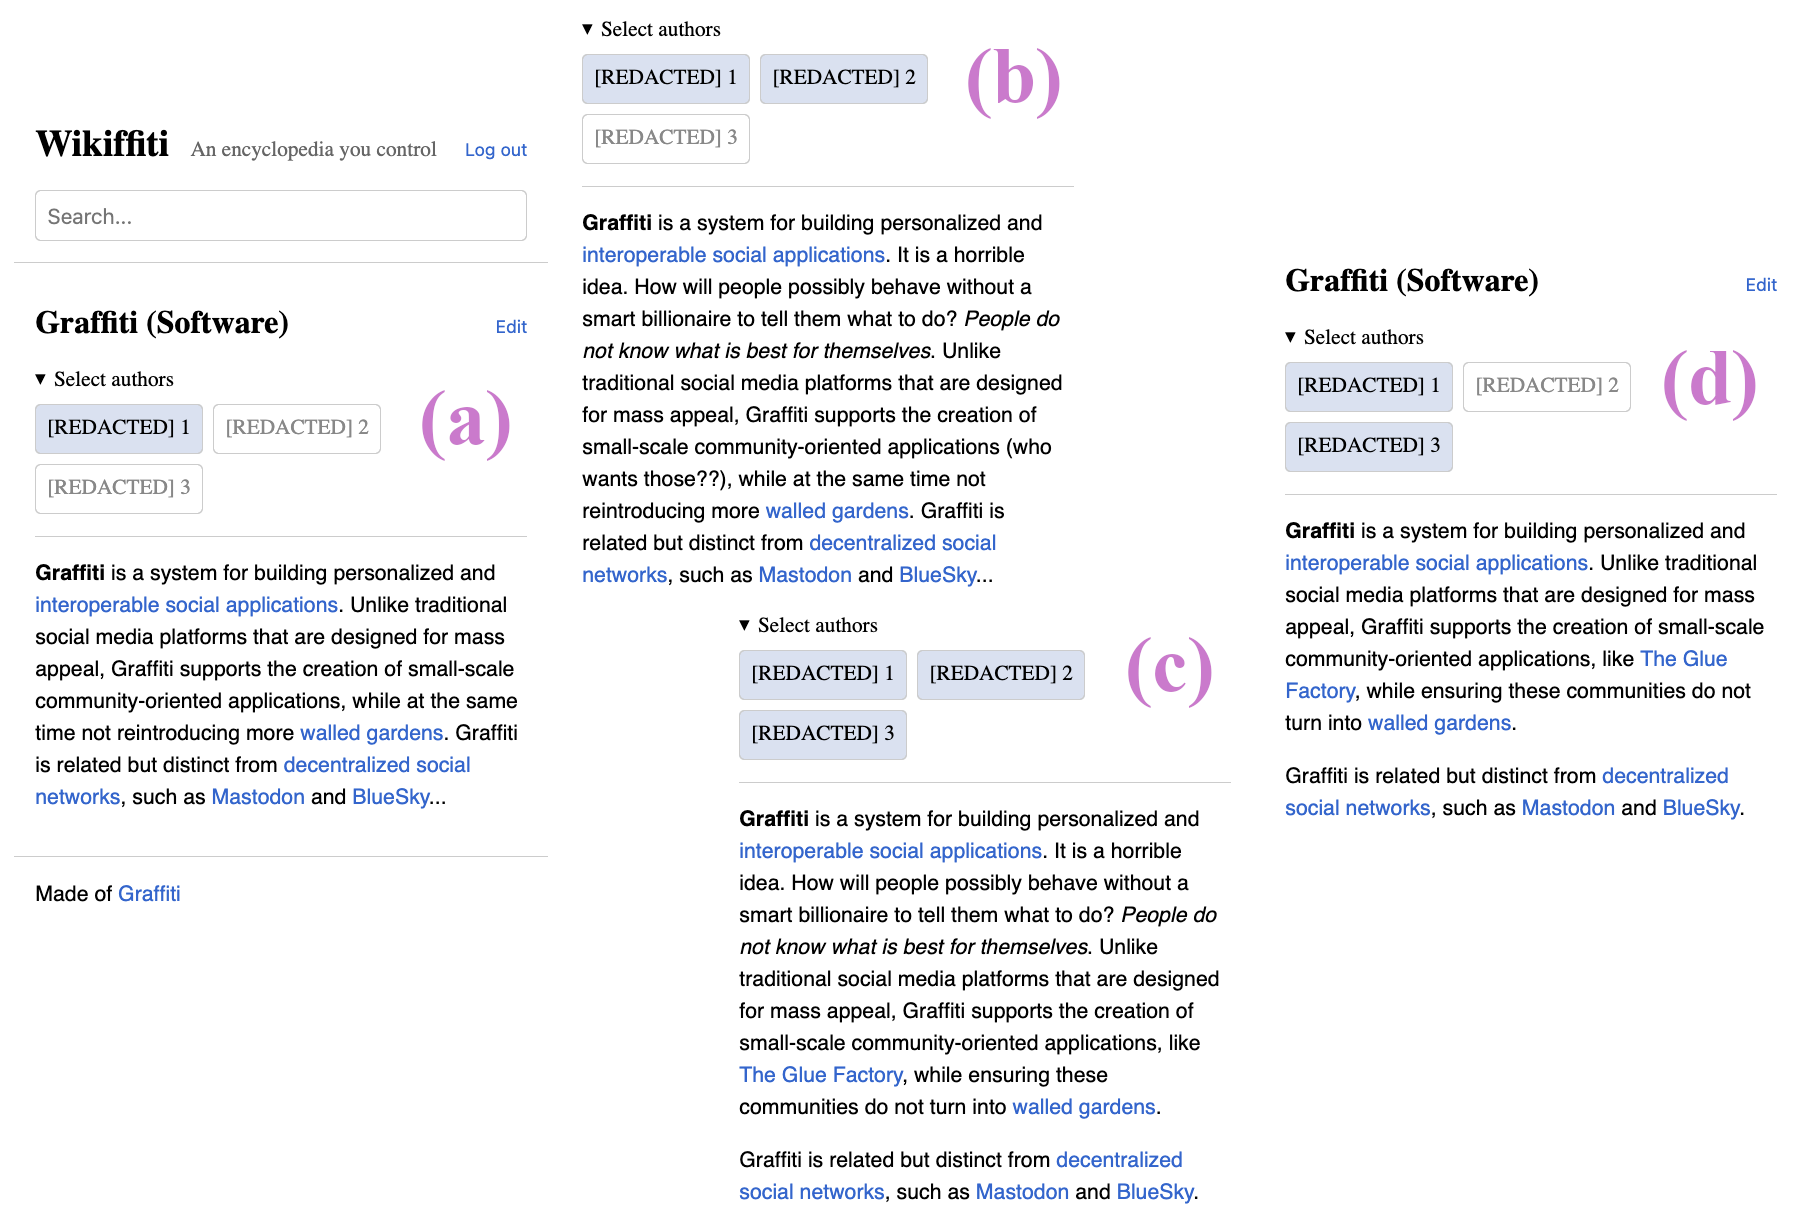
\includegraphics[width=\textwidth]{paper/figures/wikiffiti.png}
    \caption{(a) [REDACTED] 1 makes some edits to a Wikifitti page. (b) [REDACTED] 2 ``vandalizes'' the page (c) [REDACTED] 3 manually deletes some of [REDACTED] 2's edits and adds new content. (c) All of [REDACTED] 2's edits are retroactively removed.
    }

    \label{case-studies:fig:wikiffiti}
\end{figure*}
% total reification provides every user with affordance

Edits to each Wikiffiti article are published to
the channel represented by the article's title.
This allows for basic exact-match ``search'' on titles and, like on Wikipedia,
``disambiguation'' pages can serve as manual search indexes when necessary.

Edits are published and composed together according to Logoot,
a conflict-free replicated data type (CRDT)~\cite{logoot,crdts}.
Logoot, and CRDTs in general, were developed for asynchronous collaborative editing
but, luckily for us, Logoot produces reasonable results when
some edits are ``dropped,'' as we do here intentionally.
Currently, our implementation is inefficient with a 40x space blowup;
however, there are plenty of existing optimizations that one could apply~\cite{logootbetter}
and release as part of a standard collaborative editing library.

Like Parallax, Wikiffiti is an extreme. Clearly not every user
has the expertise or desire to vet all the editors of
every article they read. In reality, the work of approving editors
or individual edits will be delegated to
a hierarchy of user access levels,
friend-of-a-friend networks of trust,
or automatic vandalism detectors, for example.
Still, the data underneath can always be reinterpreted, allowing
for new systems to independently evolve that,
for example, might be more welcoming to newcomers~\cite{wikibourgeoisie, wikirisedecline}
or promote edits made by women and non-binary people~\cite{wikigender}.
An application could even highlight edits that are vandalism to some,
but art to others: graffiti.


% Vandalism to some may be empowering to other.

% All the while, maintaining the dissonance that what is vandalism to some,
% may be art to others.
